\documentclass[a4paper,10pt]{article}
\usepackage[utf8x]{inputenc}
\usepackage{amsmath}
\usepackage{graphicx}
\usepackage[english]{babel}
\usepackage{url}
\usepackage{epstopdf}
\usepackage{subfig}
\usepackage{graphicx}

\title{Procesamiento Avanzado de Imágenes\\IEE3784}
\author{\textbf{Tarea 02}\\Norman F. Sáez\\nfsaez@uc.cl}
\date{\today}

\begin{document}
\maketitle
\section{Pregunta 1}
\begin{figure}[ht!]
  \centering
  \subfloat[Cluster no supervisado]{\label{fig:img1a}\includegraphics[width=0.50\textwidth]{img/clusters.eps}}
  ~ 
  \caption{Cluster no supervisado}
  \label{fig:p1}
\end{figure}

\section{Pregunta 2}
Sin embargo los resultados no son los esperados y se pueden ver en \ref{fig:p2}
\begin{figure}[ht!]
  \centering
  \subfloat[Snakes]{\label{fig:img2}\includegraphics[width=0.80\textwidth]{img/snake.eps}}
  ~ 
  \caption{Snakes}
  \label{fig:p2}
\end{figure}
Se utilizaron 4 puntos de control y luego los cuatro siguiente, con el resultado obtenido. Como se puede apreciar claramente, no es una curva continua
por lo que lo mas probable es que no este bien aplicado el metodo. Los puntos en azul son los puntos de control de la curva.

\section{Pregunta 3}
\begin{figure}[ht!]
  \centering
  \subfloat[B-Spline, Casteljau: Puntos de control en azul]{\label{fig:img4}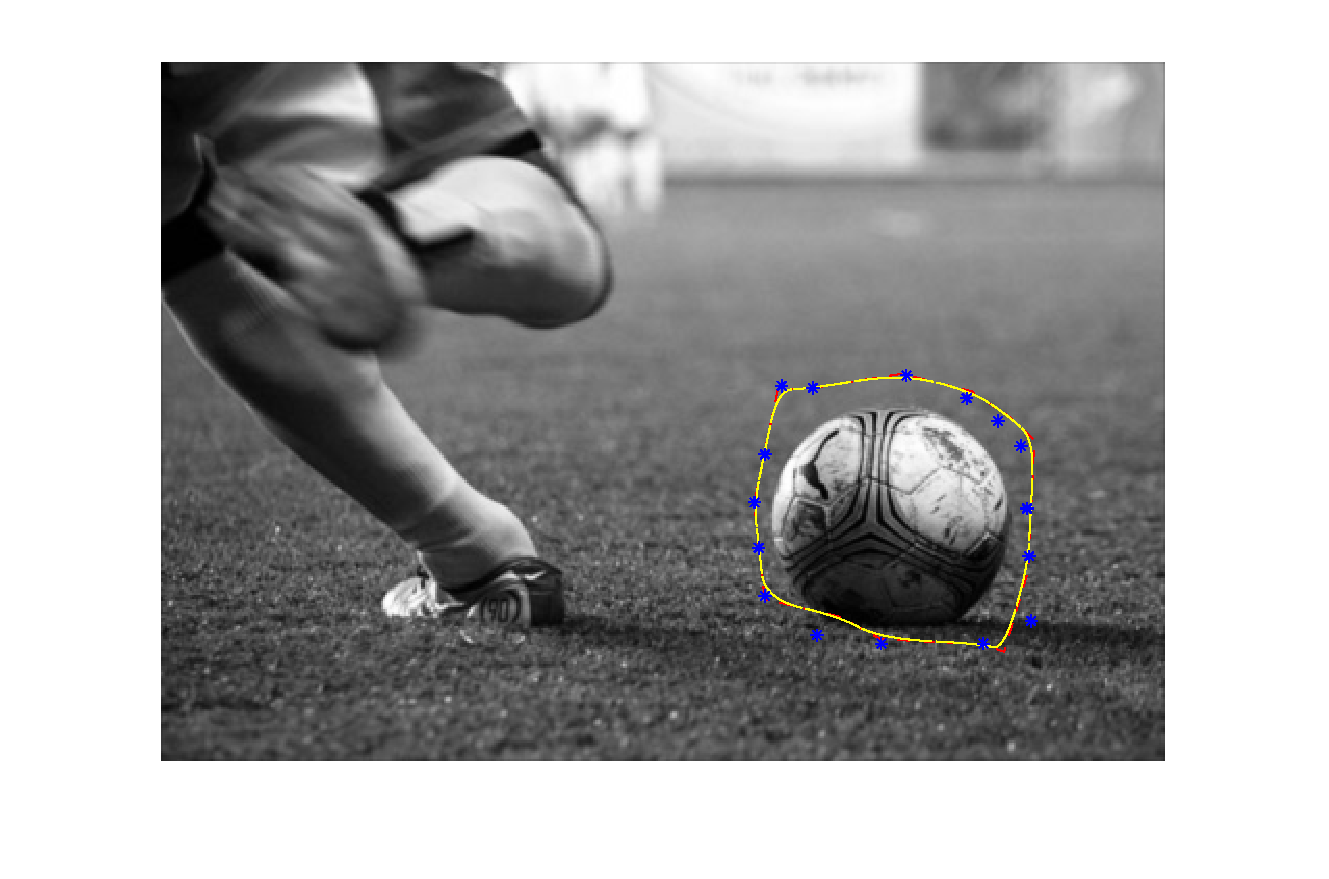
\includegraphics[width=0.50\textwidth]{img/balloon.eps}}
  ~ 
  \subfloat[B-Spline, Casteljau: Puntos de control en azul]{\label{fig:img4}\includegraphics[width=0.50\textwidth]{img/filtro_gauss.eps}}
  ~ 
  \caption{B-Splines calculado usando Casteljau}
  \label{fig:p4}
\end{figure}

\end{document}
